%第3章



\section{基本設計}

本節では感染症予防サポートシステムの全体としての動き,基本設計について述べる.

まず,システムの静的な構造を示すクラス図を図\ref{class}に示す.
\begin{figure}[htbp]
    \centering
    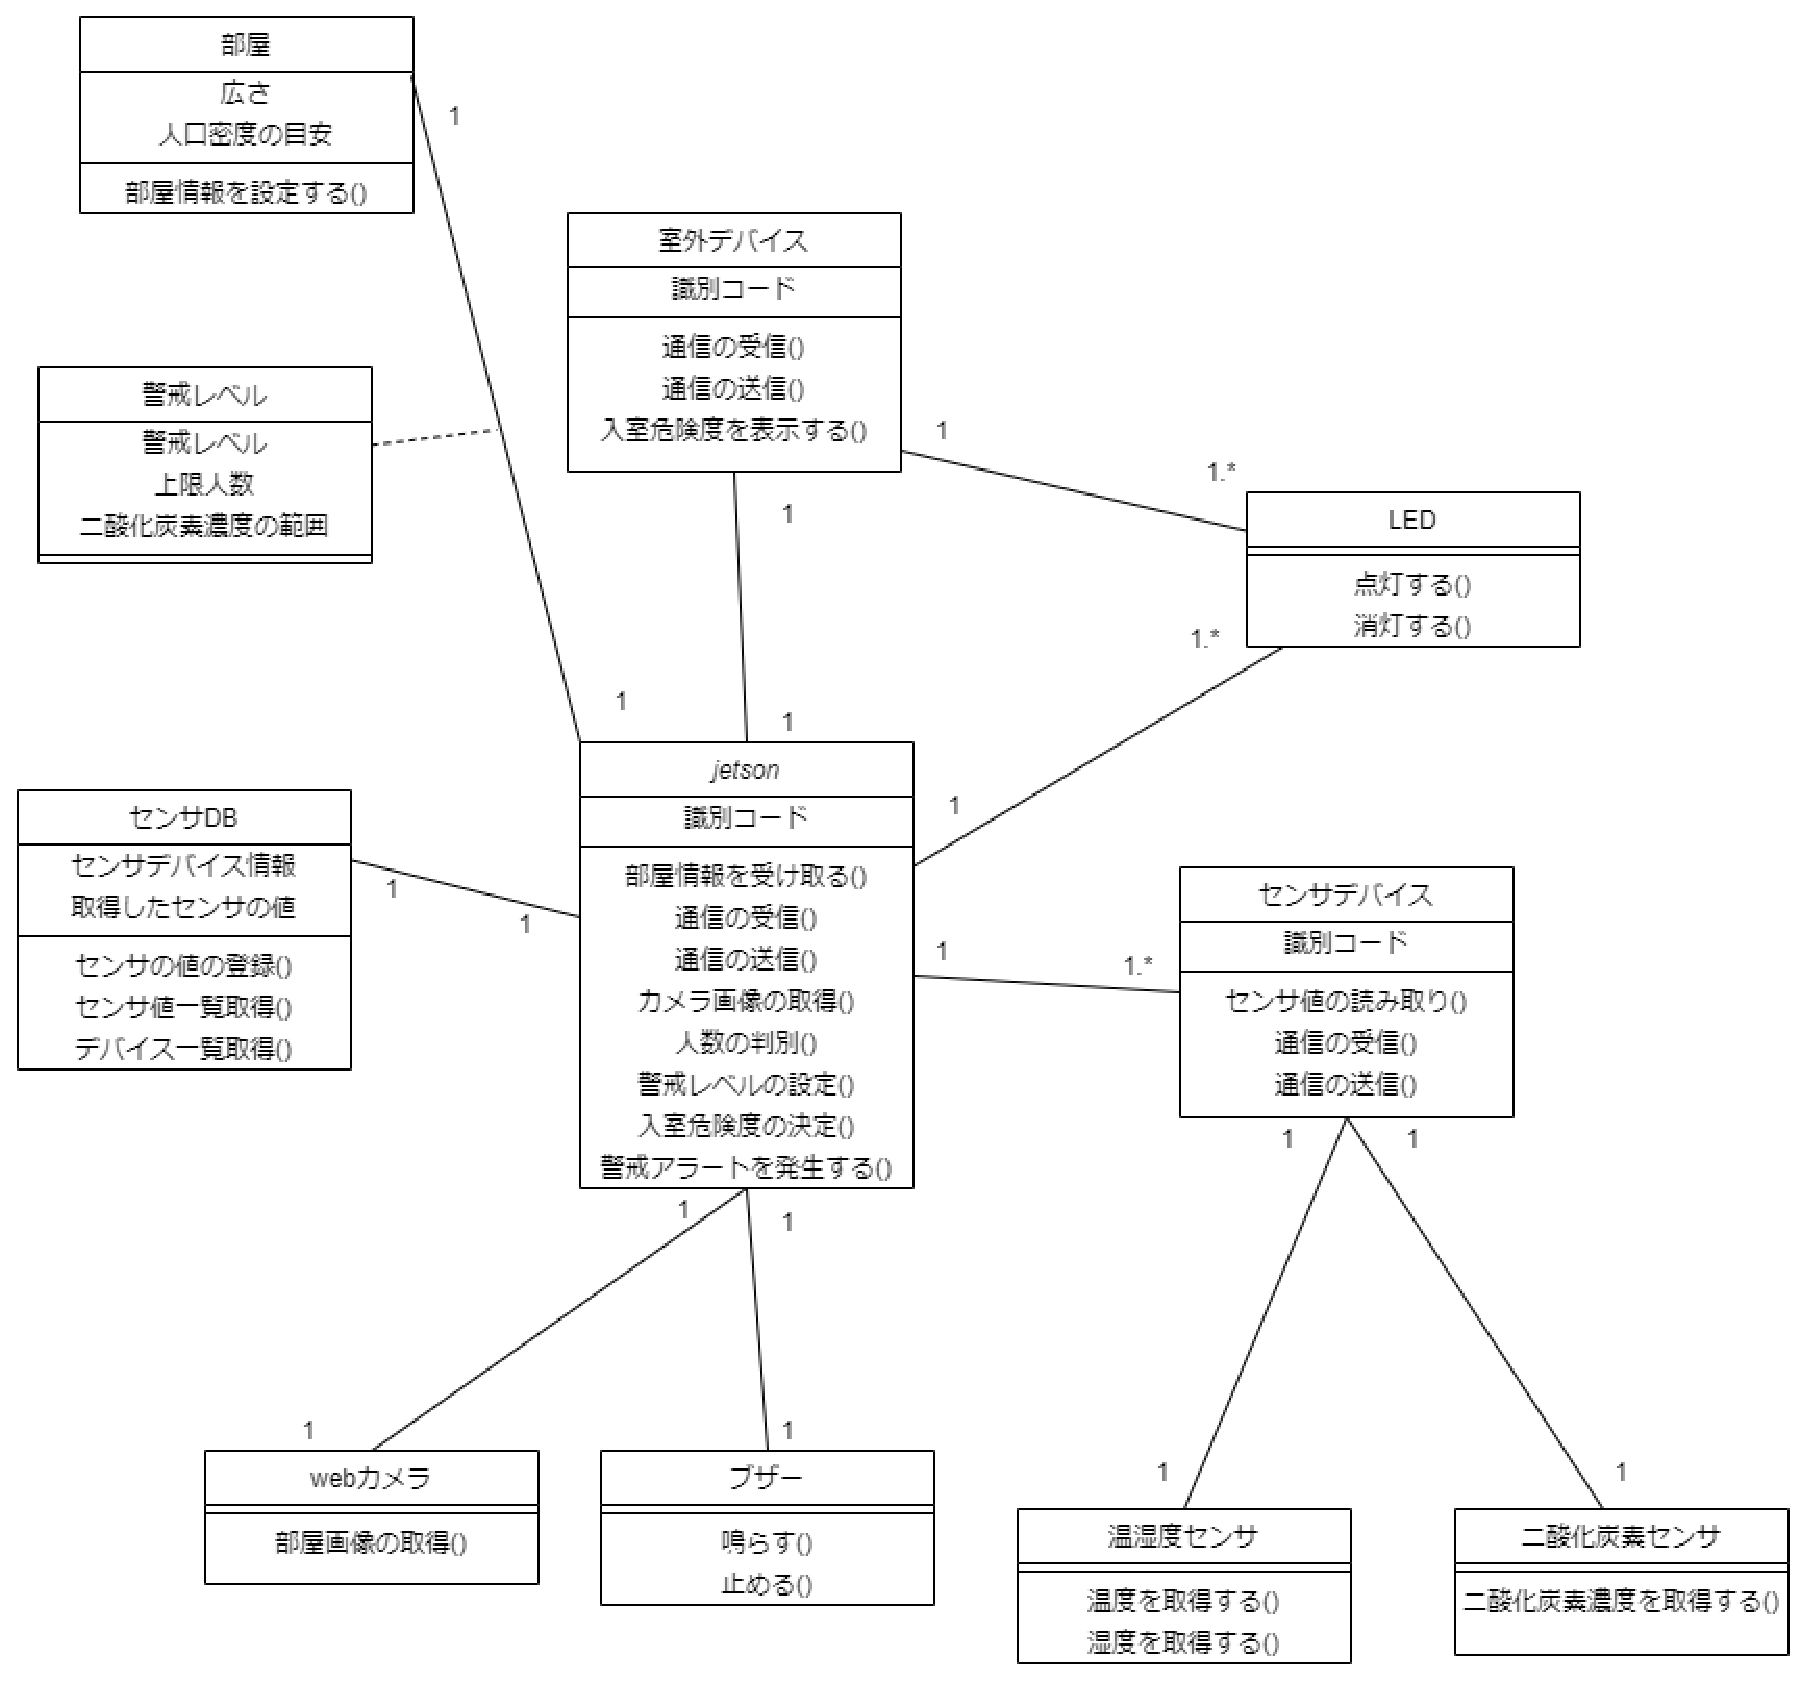
\includegraphics[width = 15cm]{./picture/class_3.eps}
    \caption{クラス図}
    \label{class}
\end{figure}
システムの構成要素としては,まず,処理などを行うJetsonクラスがある.
Jetsonひとつに対して複数のセンサデバイスクラスがあり,センサデバイスひとつに対しては温湿度センサと二酸化炭素センサクラスがそれぞれひとつずつ存在する.
また,屋外デバイスがJetsonひとつに対してひとつ存在する.
屋外デバイスは複数のLEDを持つ.
Jetsonも複数のLEDを持つとともに,ひとつのブザー,ひとつのWebカメラを持つ.
また,処理を行うJetsonクラスに対して,部屋情報,警戒レベルクラス及びデータベースであるセンサDBクラスが関係する.
Jetsonはシステムにおける各機器の取りまとめ,環境値評価の働きを担う.
Jetsonは部屋情報の読み込みを行い,部屋の広さおよび団体で設定されているガイドラインを把握する.
また,センサデバイスから受信した情報をセンサDBに記録するとともに,室内状況の評価の際にその情報を記録する.
ほかにも,Webカメラから画像の取得を行い部屋の中の人数推定を行い,室内状況の評価に用いる.
また,ブザーとLEDにより,室内の人に環境値評価に基づき警告や換気要請などを発する.
警戒レベルは,その部屋の特性を表すために利用するクラスである.
警戒レベルは,その部屋の換気のしにくさを表すものであり,そのレベルがあがると部屋状況の評価に用いる滞在推奨人数を減らしていく.
警戒レベルは部屋の二酸化炭素濃度に基づいて決定される.
センサデバイスはJetsonから指示を受け,温湿度および二酸化炭素濃度を計測するとともにその情報を送信する.
室外デバイスはJetsonからの指示を受け,入室危険度の表示のため室外に設置されているLEDの点灯,消灯の操作を行う.


続いて,システムの各機能の処理の流れをアクティビティ図を用いて説明する.
「室内状況を監視する」アクティビティ図を図\ref{act_kanshi}に,
「入室危険度の確認」のアクティビティ図を図\ref{act_enterlisk}に,
「換気要請の受け取り」のアクティビティ図を図\ref{act_kanki}に,
「室内環境状態の表示」のアクティビティ図を図\ref{act_kankyou}に示す.
\begin{figure}[htbp]
    \centering
    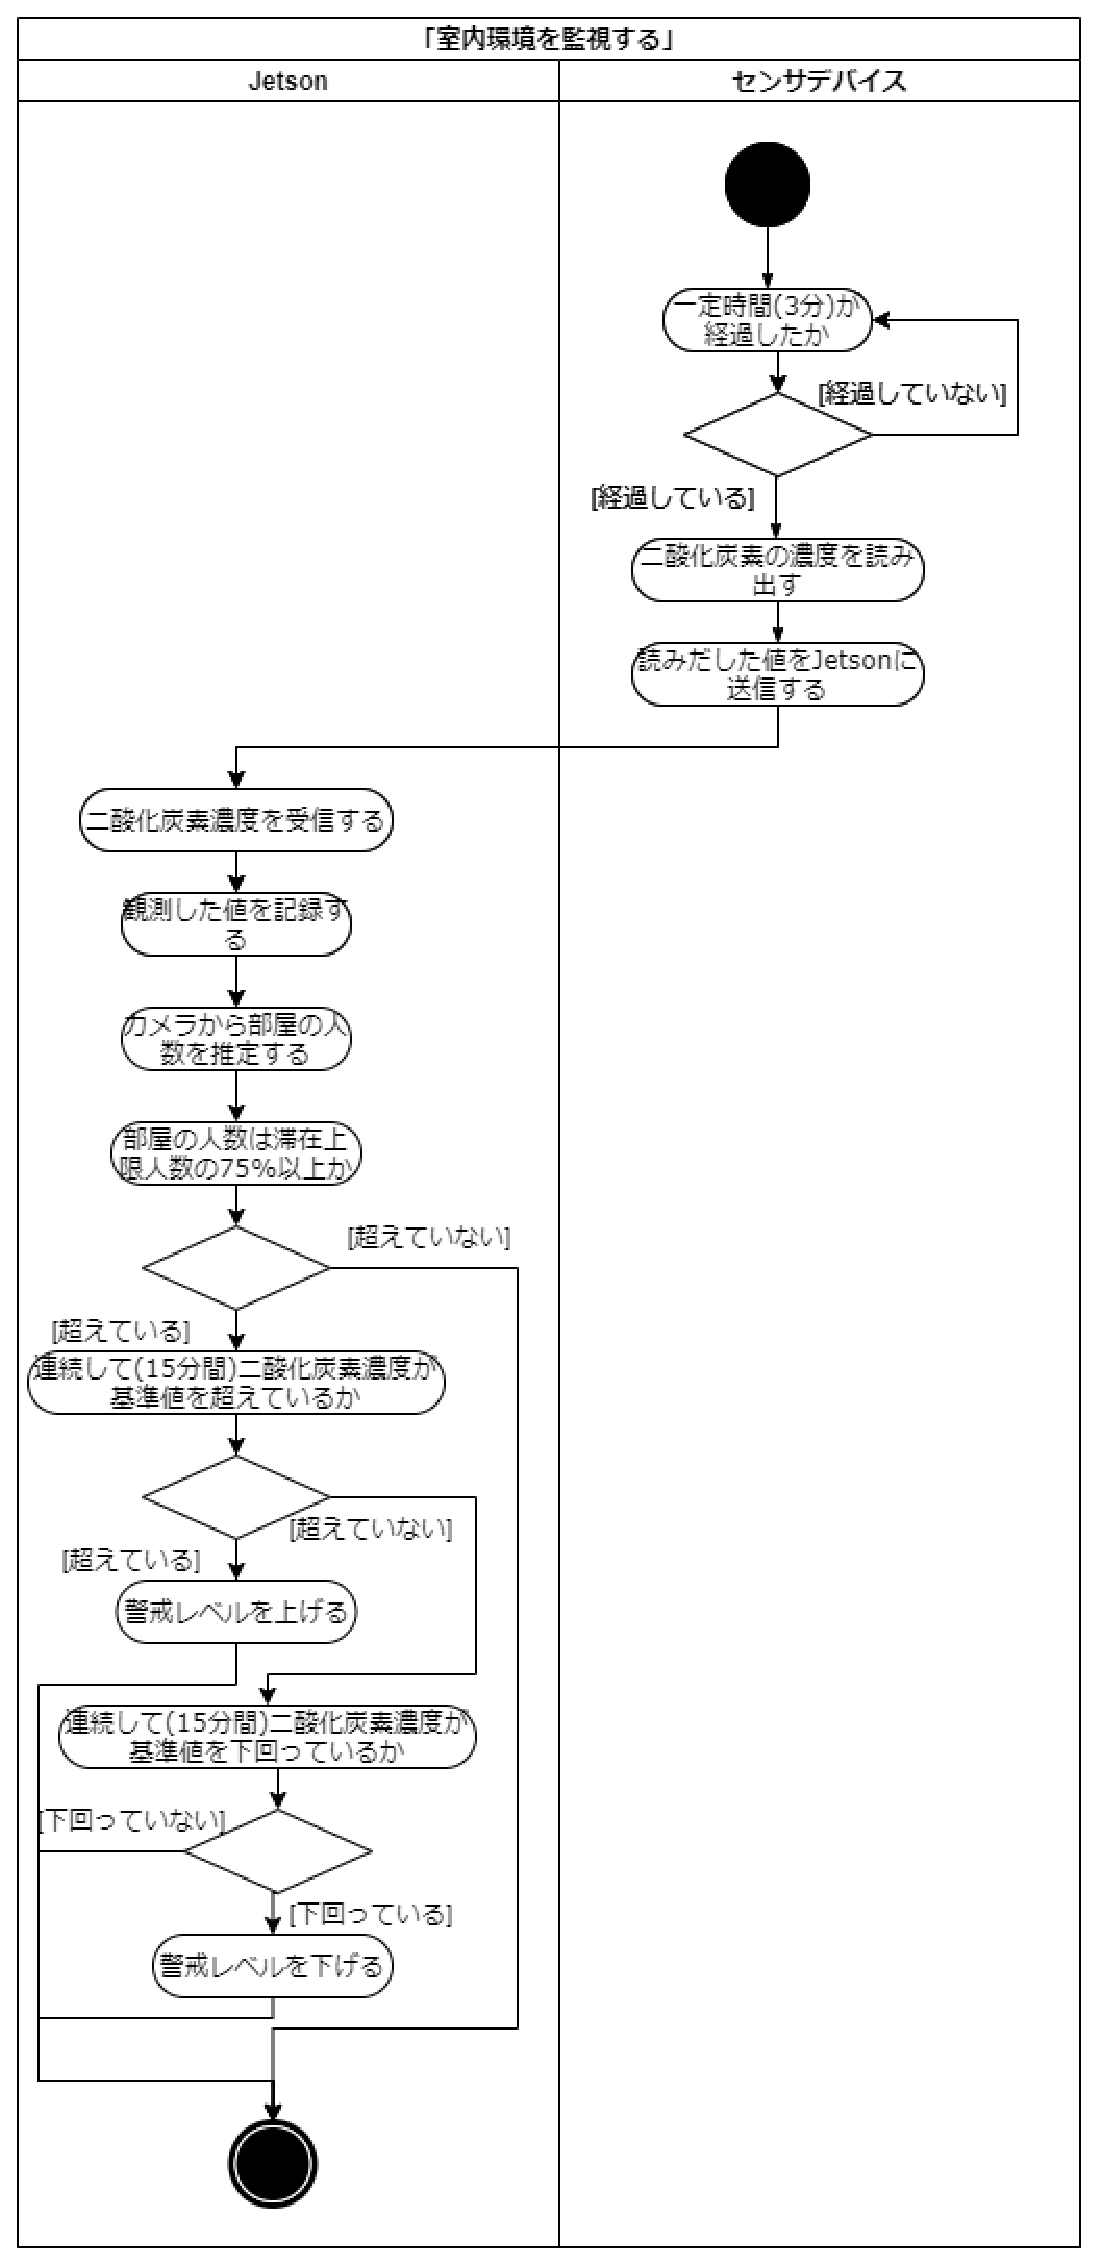
\includegraphics[width = 9cm]{./picture/activity_kanshi_1.eps}
    \caption{ユースケース「室内状況を監視する」のアクティビティ図}
    \label{act_kanshi}
\end{figure}
\begin{figure}[htbp]
    \centering
    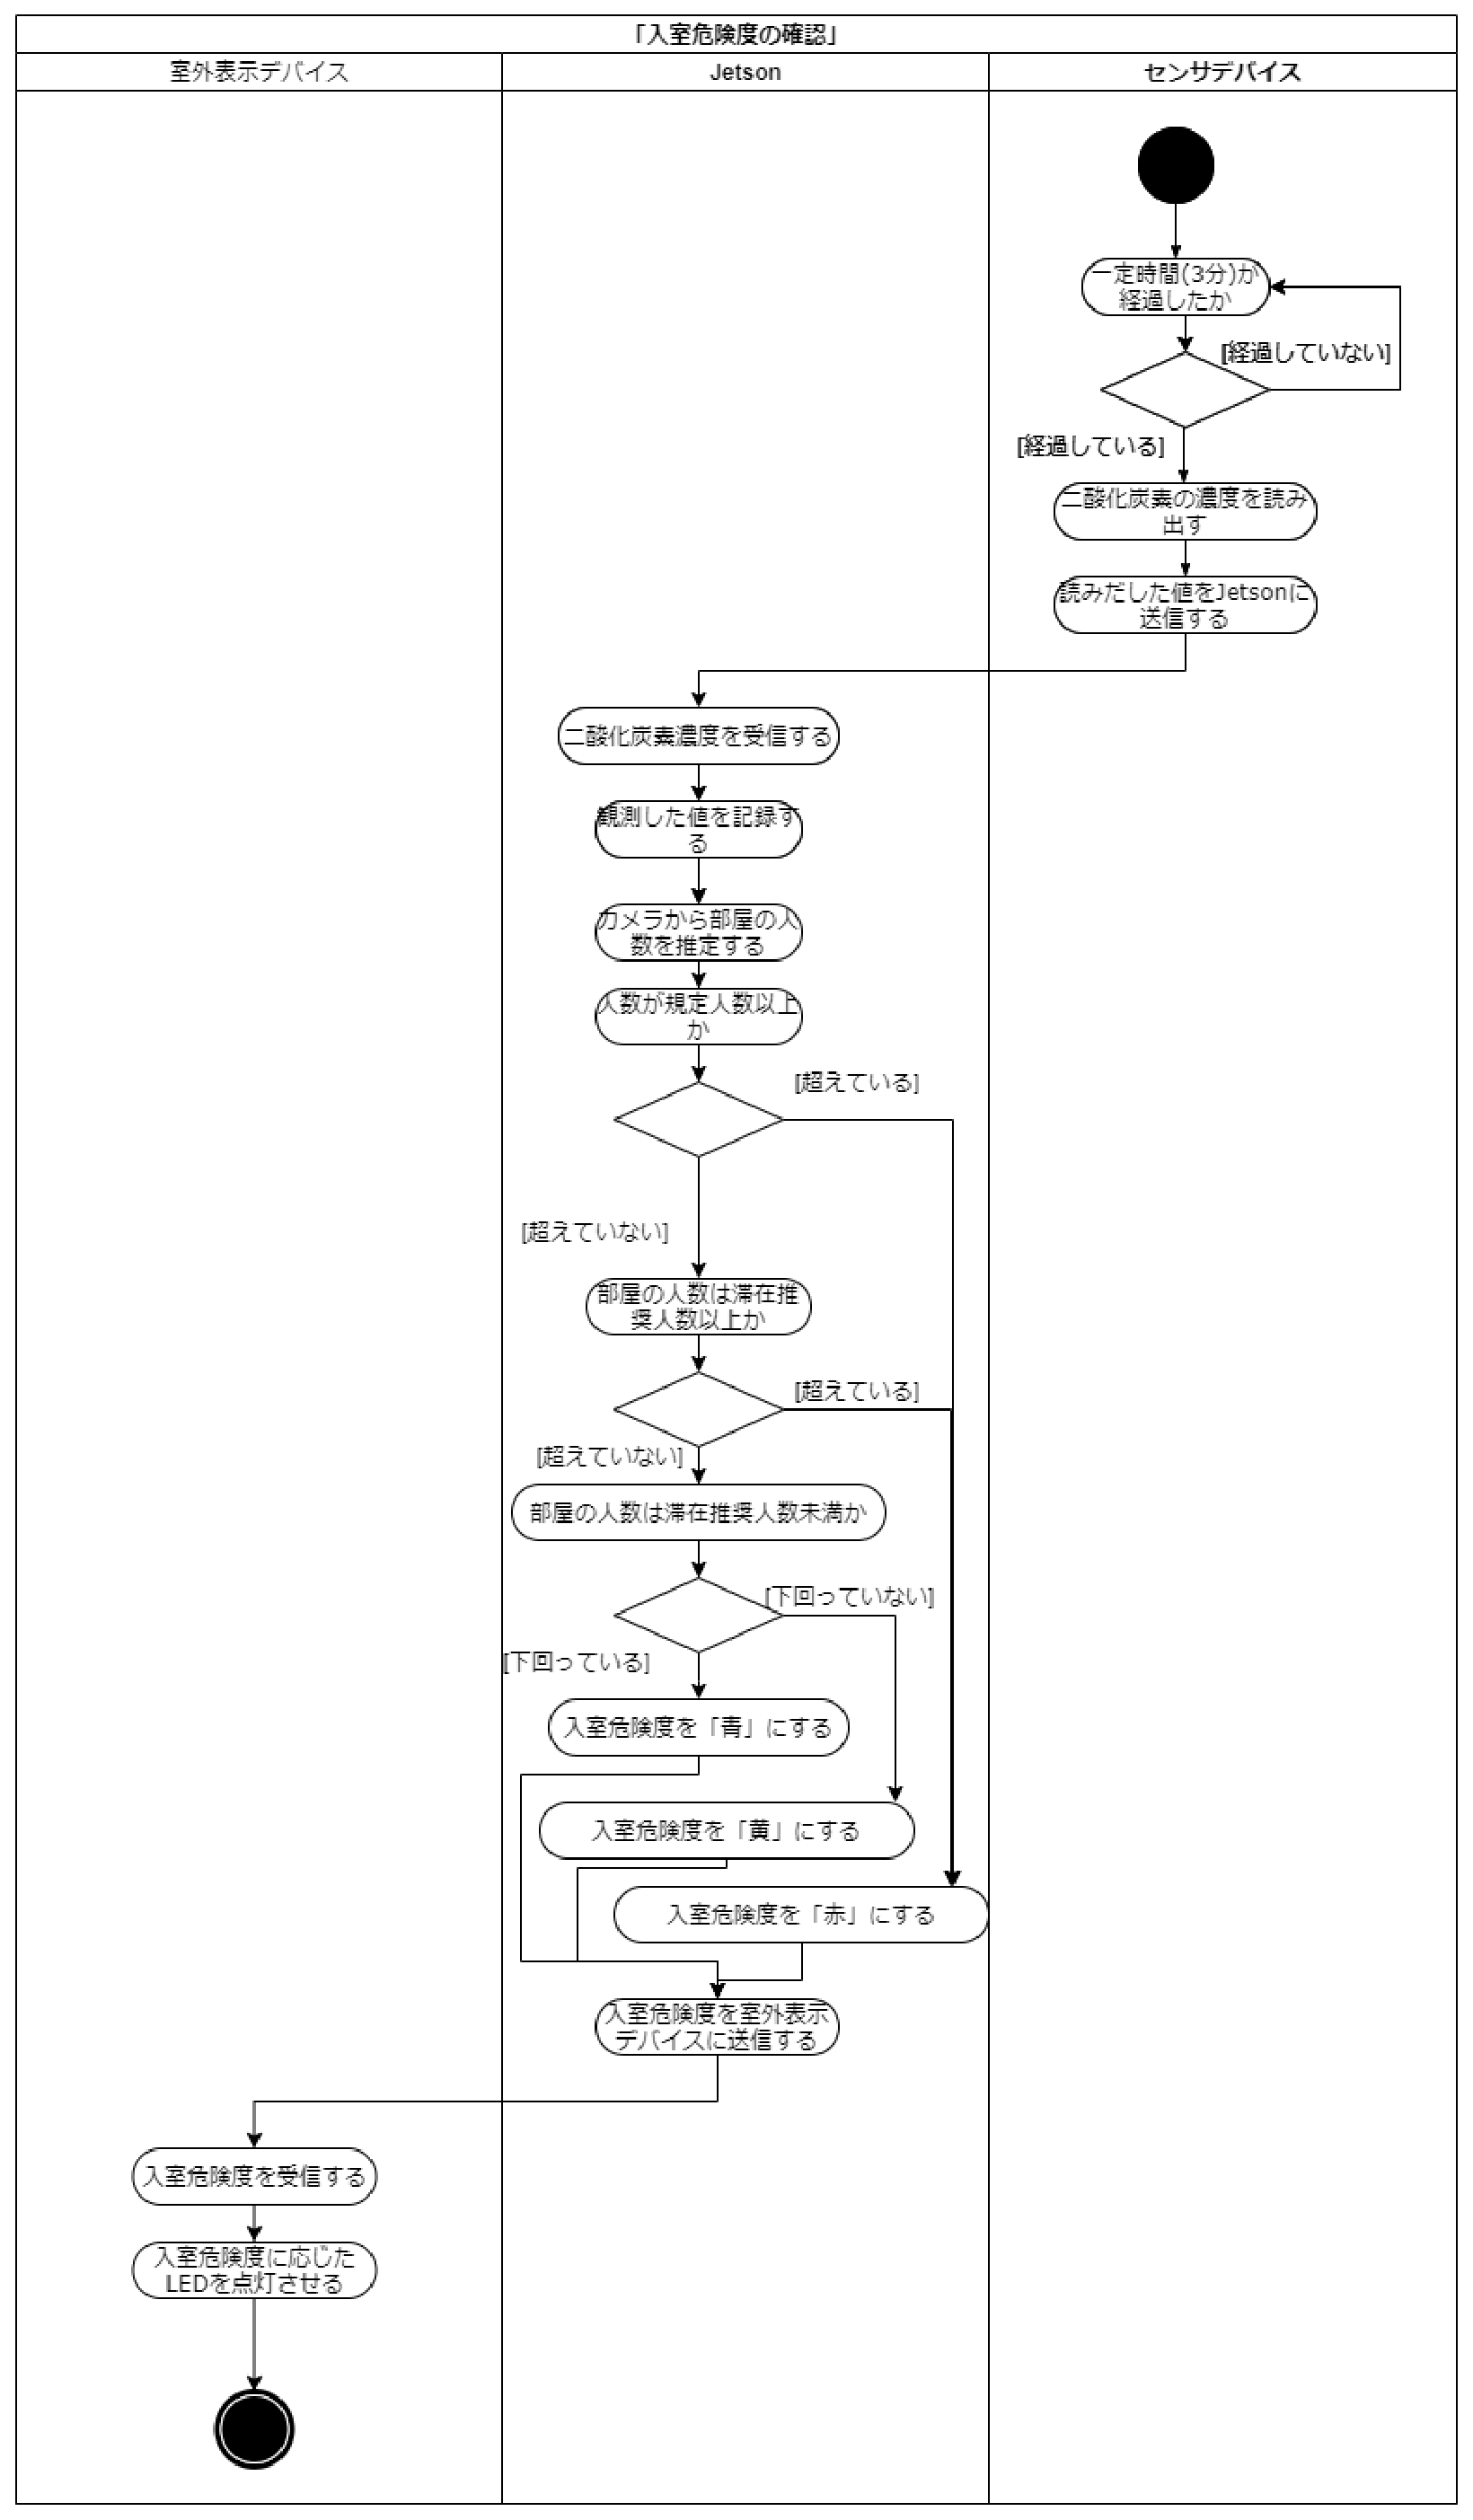
\includegraphics[width = 12cm]{./picture/activity_enterlisk_1.eps}
    \caption{ユースケース「入室危険度の確認」のアクティビティ図}
    \label{act_enterlisk}
\end{figure}
\begin{figure}[htbp]
    \centering
    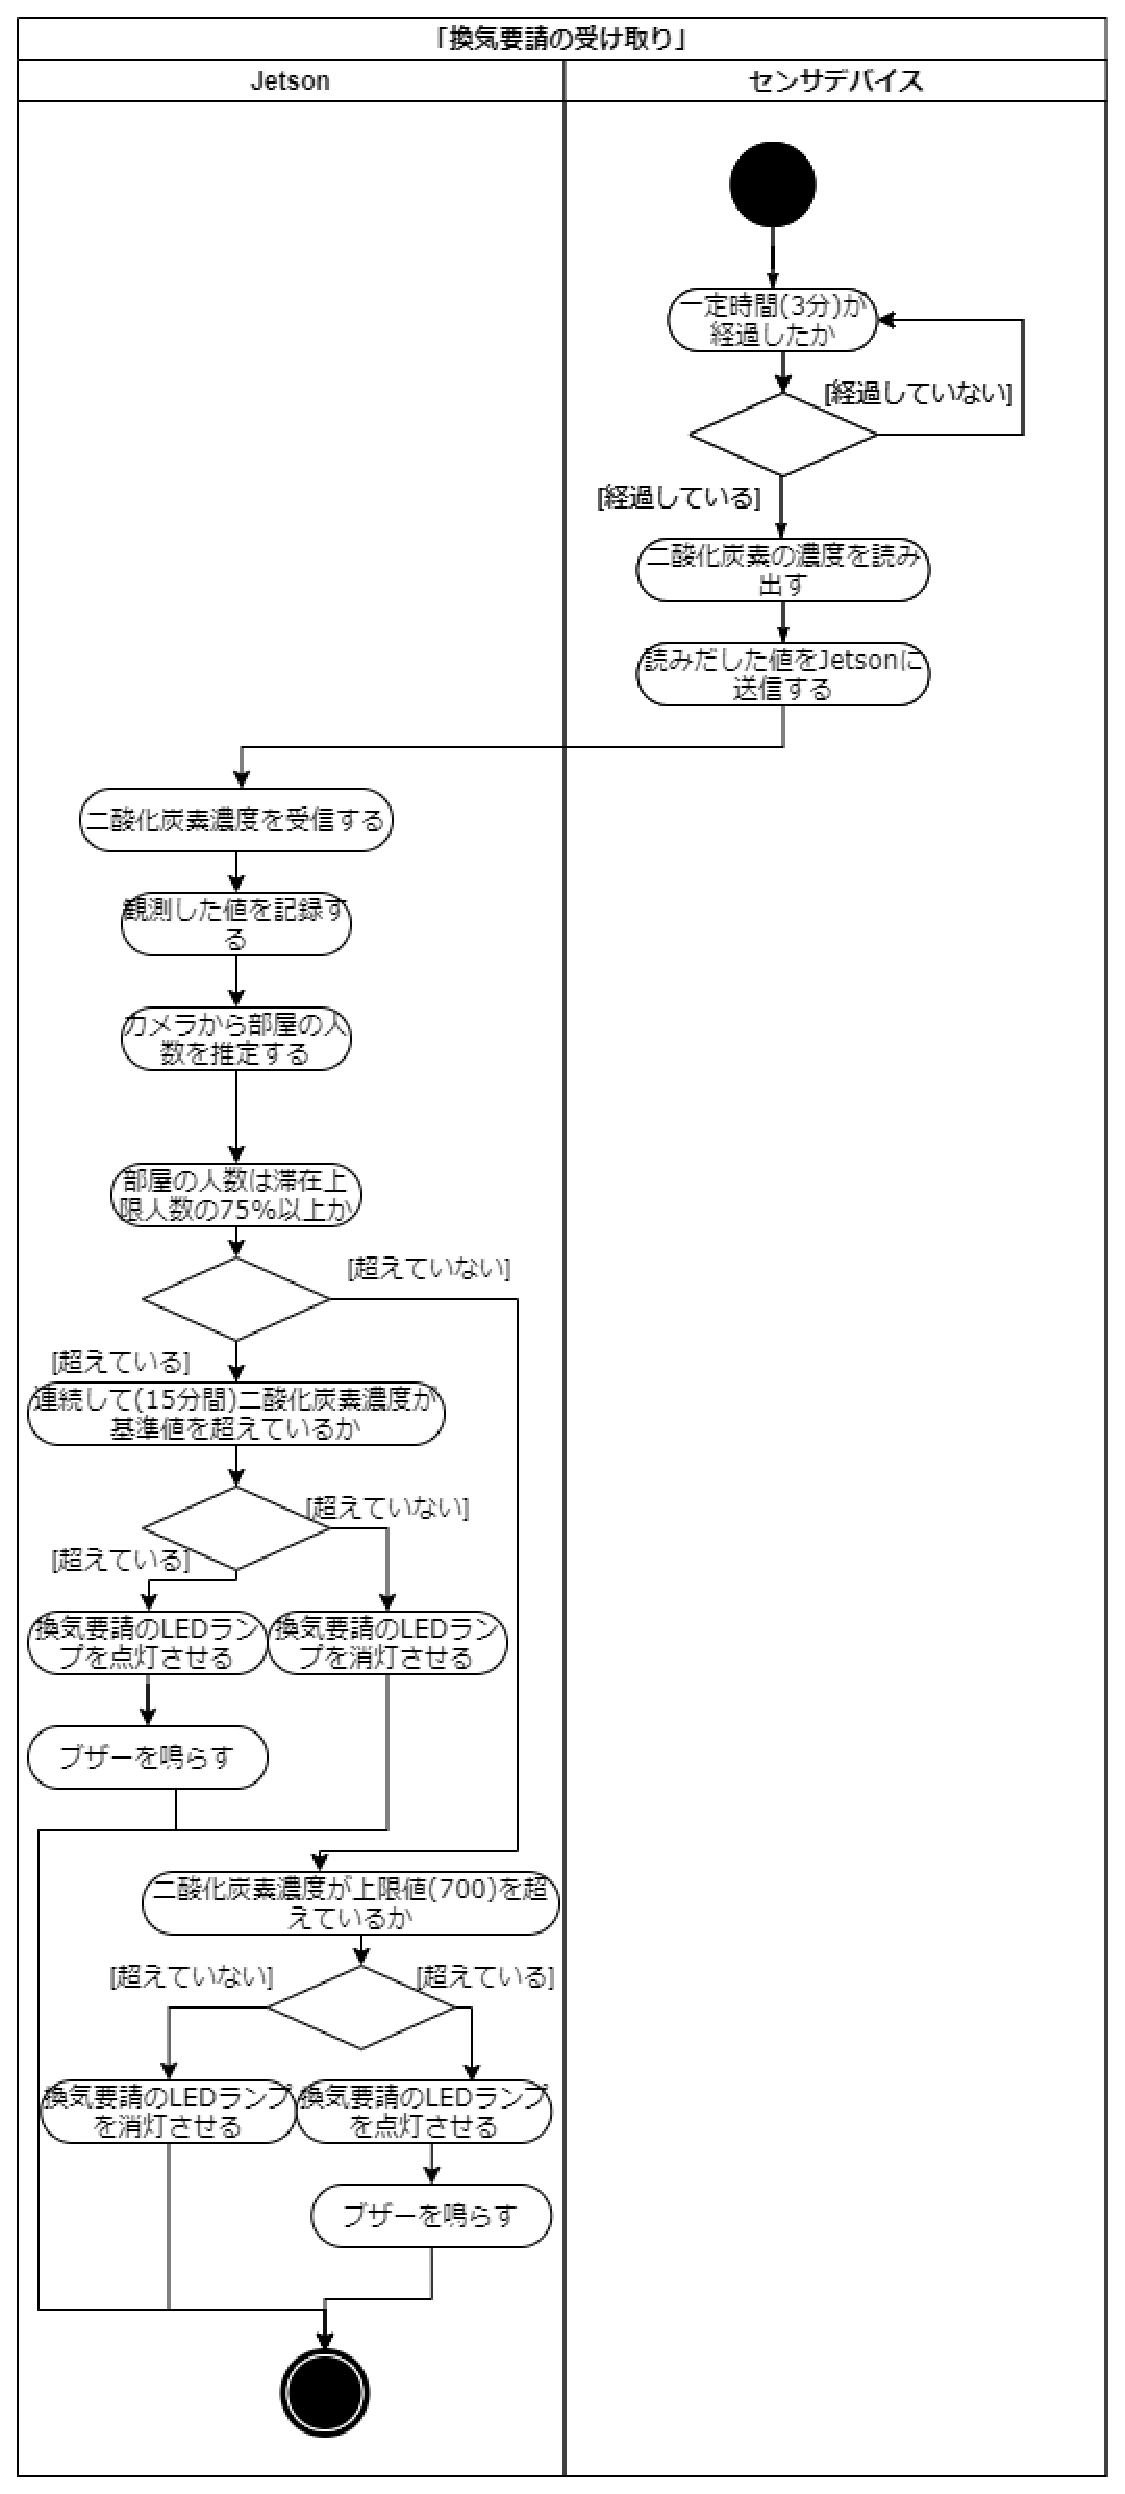
\includegraphics[width = 9cm]{./picture/activity_kanki_1.eps}
    \caption{ユースケース「換気要請の受け取り」のアクティビティ図}
    \label{act_kanki}
\end{figure}
\begin{figure}[htbp]
    \centering
    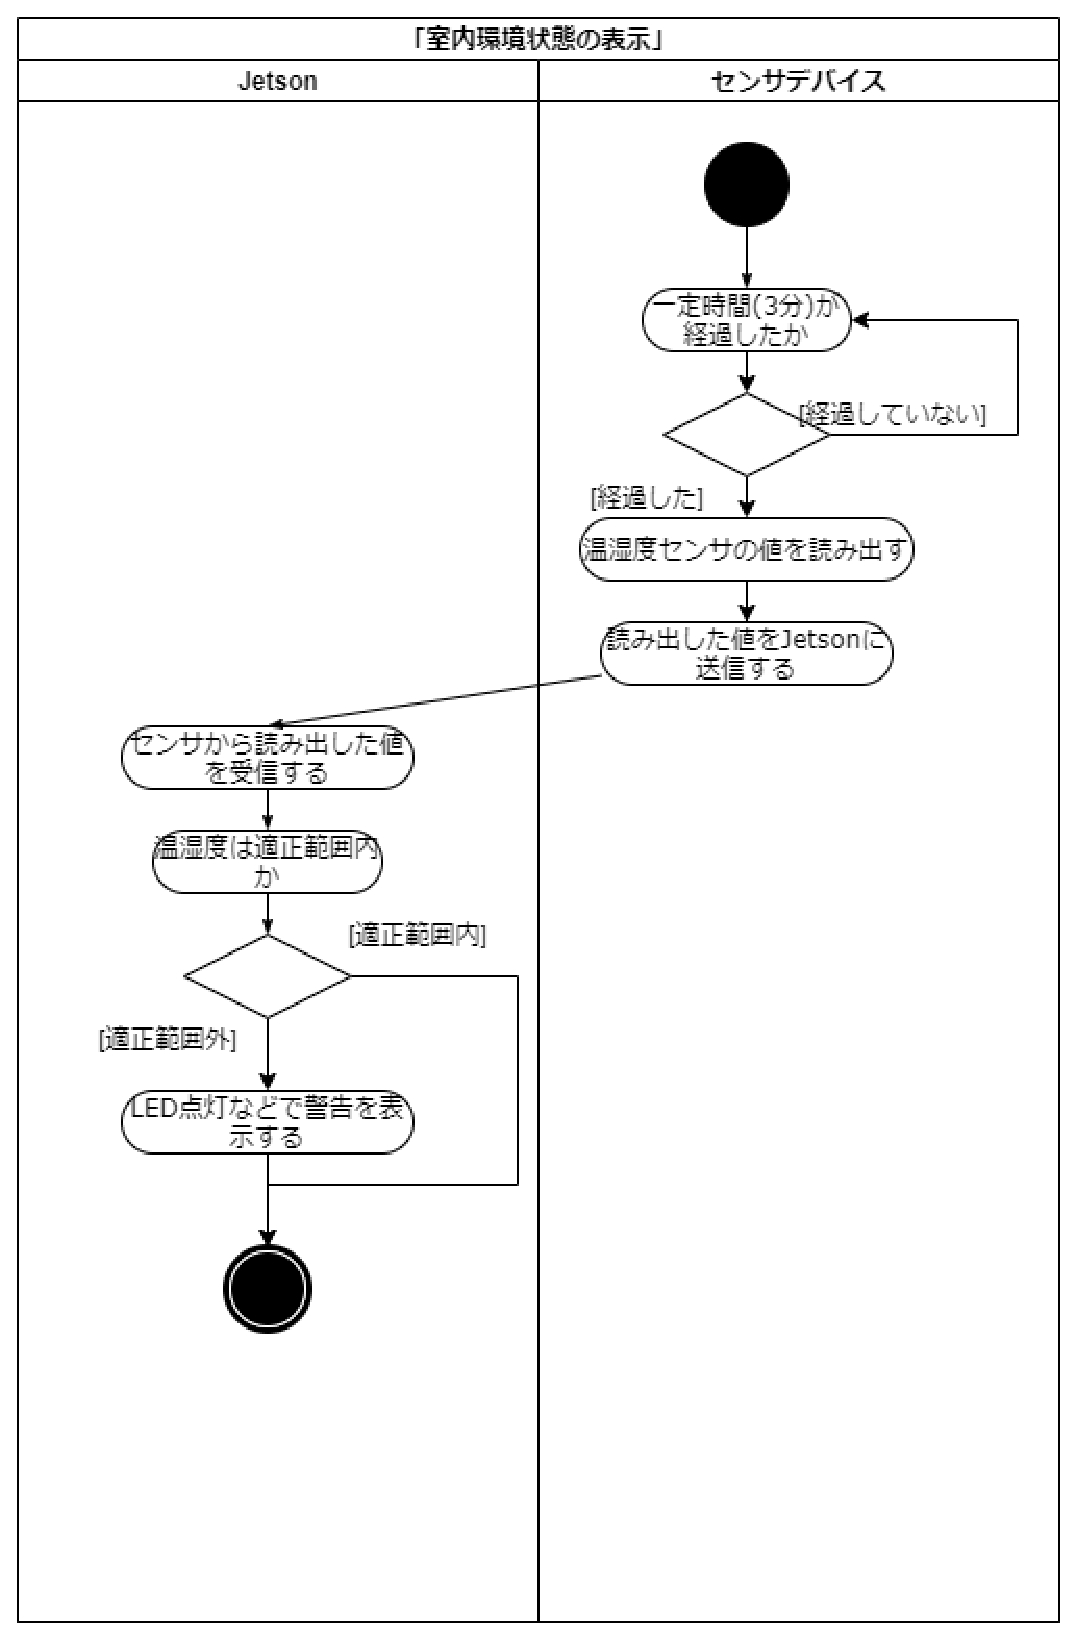
\includegraphics[width = 9cm]{./picture/activity_kankyou_2.eps}
    \caption{ユースケース「室内環境状態の表示」のアクティビティ図}
    \label{act_kankyou}
\end{figure}

まず,「室内状況を監視する」というユースケースについて説明する.
これは,一定時間ごとに部屋の人数推定および二酸化炭素濃度計測を行うことで,部屋の警戒レベルの調整を行うものである.
一定時間とは,ここでは3分おきに実行するものとした.
3分ごとにセンサデバイスで二酸化炭素濃度を読み出し,読みだした値をJetsonに送信する.
Jetsonではそれを受信し,部屋の人数推定をWebカメラを用いて行う.
その後,人数が部屋の滞在上限人数の75\%以上となっていた場合,二酸化炭素濃度を用いて警戒レベルの上げ下げを行う.
ここで人数が75\%以上の時のみ警戒レベルの計算を行うというのは,部屋に人があまりいない場合警戒レベルを増減させてしまうと,警戒レベルが部屋の特性に関係なく,必要以上に低いものとなってしまうのを防ぐためである.

続いて,「入室危険度の確認」というユースケースについて説明する.
これも3分おきに実行され,部屋の人数をもとに入室危険度を設定する.
3分の経過確認,人数推定を行うまでは上記「室内状況を確認する」ユースケースと同様である.
その後,学校や団体のガイドラインで制定されている規定人数,警戒レベルの滞在推奨人数をもとに入室危険度を「赤」,「黄」,「青」の三種類で判定する.
入室危険度については,信号機の色の使い分けを参考にし,最も危険な状態を「赤」,最も安全な状態を「青」,その中間を「黄」として表現している.
最後に,その入室危険度を室外表示デバイスの対応した色のLEDを点灯させることにより表示する.

「換気要請の受け取り」のユースケースについて説明する.
ここでは,二酸化炭素濃度と部屋の人数推定の結果を用いて換気要請の判断,表示を行う.
二酸化炭素濃度,部屋の人数推定については上記「室内状況を監視する」ユースケースと同様に行われる.
その結果,部屋の人数が滞在上限人数の75\%以上かどうかを判断する.
部屋の人数が少なかった場合にはビル管理法で定められている目安である二酸化炭素濃度が1000ppmを超えているかを確認し,換気要請を行う.
一方,部屋の人数が多い場合には,法律のものより厳しく設定した警戒レベルの基準値に従い,換気要請を行う.
換気要請を行う際には,LED点灯のみだけでは気づきにくい場合があるので,ブザーも同時にならす.

最後に,「室内環境状態の表示」のユースケースについて説明する.
これは,一定時間ごとに部屋の温湿度の値を収集し,適正値から逸脱した場合にそれを通知するものである.
この通知による改善要求ついては,換気に比べ,緊急性が低いと考えられるため,LEDの点灯のみで通知することとした.

上記の設計を受け,結合テストのテスト項目を表\ref{ketugoutest_koumoku}の通り作成した.
\begin{table}[htbp]
    \centering
    \caption{結合テスト項目}
    \label{ketugoutest_koumoku}
    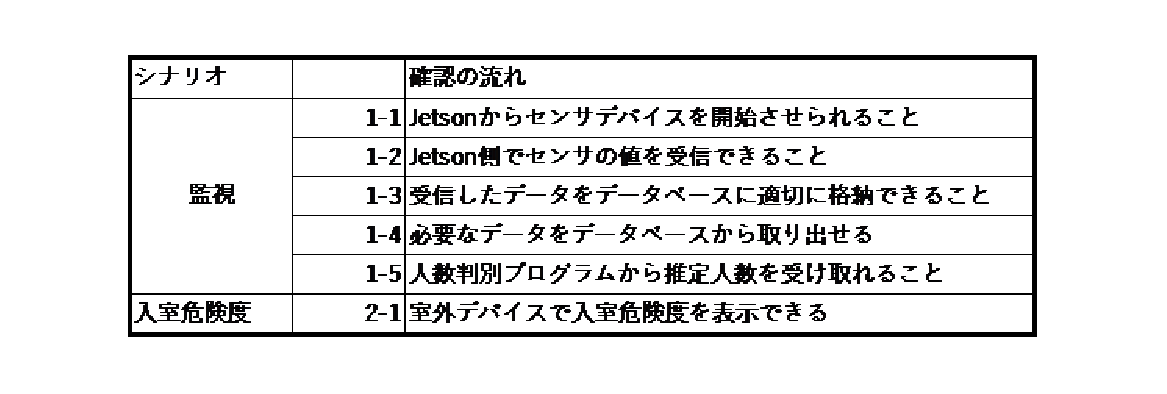
\includegraphics[width = 15cm]{./picture/ketugoutest_koumoku.eps}
\end{table}

\subsection{使用部品・モジュールの選定}
基本設計の段階において使用する各部品・モジュールの選定を行った.
下記に私が担当したセンサデバイスで使用したものと,それぞれの選定理由を述べる.

センサデバイスのマイコンについては,TWELITEを使用した.
このTWELITEは,モノワイヤレス株式会社の無線マイコンである\cite{twelite}.
センサデバイスについてはJetsonと通信を行う必要があり,通信機能を搭載した,もしくはモジュールとしてその機能を追加できるマイコンボードを使用する必要がある.
通信においては,設置場所への制約を少なくするため,コードの配線を考えなくてもよい,無線を利用することとした.
無線規格については様々存在するが,本システムではIEEE802.15.4を用いることとした.
無線機能については,マイコンボードにすでに実装されているものと,マイコンボードとは別にモジュールを接続する必要があるものが存在する.
本システムではデバイスを小さくできるため,マイコンボードに無線機能があらかじめ実装されているものを用いることとした.
また,センサデバイスは,設置場所の制約を少なくするため,通常のバッテリーと比べ比較的小さく,かつ一般的に手に入りやすく交換が容易にできる乾電池で動作できることが必要であるとした.
乾電池は一般的に起電力1.5Vであるが,1.5Vで動作するマイコンボードはほとんどなく,センサモジュールについても最低3V程度必要なものが多いため,2本使用し,3Vで動作するものを利用することとした.
以上の理由より,起電力3Vで動作し,IEEE802.15.4が実装されているマイコンボードとして,TWELITEを選定した.
なお,Jetsonでセンサデバイスとの電波送受信を行うモジュールとしても同じくTWELITEを選定した.
理由としては,JetsonのGPIOの基準電圧である3.3Vで動作し,かつUART接続により通信が可能であるためである.
センサデバイスと合わせ,Jetsonの送受信モジュールとして用いるTWELITEの実装についても私が担当した.

ここで,無線規格としてIEEE802.15.4を選定した理由を述べる.
無線規格はIEEEが中心となり標準化が進められており,無線製品のほとんどはこの規格に準拠したものとなっている.
本システムでは,部屋の中,および部屋の周辺のみでしか通信を行わないため,近距離無線を定義したIEEE802.15を中心に検討を行った.
その中でも普及が進んでおり,特によく利用されるものは,IEEE802.15.1,IEEE802.15.4である\cite{wnet}.
IEEE802.15.1は,Bluetoothという規格でも用いられており,これは主に音声をはじめとした数Mbps程度の中速データ転送に利用される\cite{wnet}.
IEEE802.15.4は,IEEE802.15.1と比べ速度は遅いものの,省電力であるという特徴をもつ.
本システムにおいては,通信でやり取りするデータは,入室危険度や二酸化炭素などの環境値のみであり,非常に少ないため,IEEE802.15.4で十分であると考えられる.
また,電池交換などの回数を減らすために,省電力で動作することが求められるため,省電力で使用できるIEEE802.15.4が適切であると考え,この規格に準拠したものを使用することとした.

温湿度センサについては,TWELITEが対応している接続規格で接続でき,かつ一般的に入手しやすいものとしてBOSCH社のBME280を選定した.
このセンサは電圧3Vで動作が可能であり,通信規格として$I^2C$でTWELITEと通信できるため,このセンサを選定した.
二酸化炭素濃度センサについては,一般的に入手しやすく,かつTWELITEと通信ができるものとしてZhengzhou Winsen Electronics Technology社のMH-Z14Aを選定した.
これは,アナログ電圧出力,およびUART規格によってTWELITEと通信可能であるため選定した.
二酸化炭素濃度センサにおいては,一般的に入手しやすいもので3Vで動作可能なものが存在しなかったため,動作電圧5Vのものを利用した.
動作電圧が異なるため,二酸化炭素濃度センサにおいては昇圧モジュールを利用し,センサへの供給電圧を3Vから5Vに昇圧コントロールすることで利用することとした.





% システムの構造を論理的,静的にみるためにクラス図を作成した.以下にICタグを用いた商品識別システムのクラス図として,図\ref{class_ic}を載せる.

% \begin{figure}[htbp]
% \centering
% \includegraphics[width=15cm]{./picture/class_ic.eps}
% \caption{ICタグを用いたシステムのクラス図}
% \label{class_ic}
% \end{figure}


% 図\ref{class_qr}はQRコードを用いた商品識別システムのクラス図である.


% \begin{figure}[htbp]
% \centering
% \includegraphics[height = 9cm,width=15cm]{./picture/class_qr.eps}
% \caption{QRコードを用いたシステムのクラス図}
% \label{class_qr}
% \end{figure}


% 図\ref{class_ic}と図\ref{class_qr}の違いは,ユーザ情報の登録をユーザのICタグから行うか,ユーザの形態から行うかという違いである.本研究では,クラスとしてカート(カゴ)・解析システム・カゴDB・商品DBの部分を開発対象とした.開発対象となる部分については,ICタグを用いた場合とQRコードを用いた場合とで違いはないため,そのまま本研究で実装する優先度の高いシステムのクラス図をまとめて,図\ref{class_qr_2}に示す.


% \begin{figure}[htbp]
% \centering
% \includegraphics[width=15cm]{./picture/class_final.eps}
% \caption{高優先度のシステムのクラス図}
% \label{class_qr_2}
% \end{figure}


% 図\ref{class_qr_2}において,筆者の担当した範囲はクラスとしては「カート(カゴ)」の部分である.カゴでは各種センサの制御と,解析システムへの情報の送信を行う.カゴは画像データと追加か削除のフラグ,総重量,超音波センサの情報を保持し,解析システムへ画像データとフラグをセットにし,送信する.

% なお,優先度の高い項目部分において,結合テストの際に用いる,各実装対象のテスト項目を下記の表\ref{ketsugo}に示す.

% \begin{table}[htbp]
% \centering
% \caption{結合テスト項目}
% \includegraphics[width = 15cm]{./picture/ketsugo.eps}
% \label{ketsugo}
% \end{table}


% また,基本設計の段階で,それぞれの用途のために各種センサを選定した.下記に選定したセンサと選定理由を述べる.


% \subsection{Webカメラの選定}


% まず,バーコードを読み取る装置の選定である.3.1節に述べた基本の評価軸より,コストを抑えられるか,従来のセミセルフレジより簡単な動作で決済まで行えるかを検討した.バーコードを読み取ることができる装置であり,それに加えて拡張性のある装置かどうかを基準として選定した.コストを抑えることかつバーコードを読み取ることができる装置として,バーコードリーダー,Webカメラが挙げられる.バーコードリーダーとWebカメラを比較した表を下記表\ref{came}に示す.


% \begin{table}[htb]
% \begin{center}
% \caption{バーコードリーダーとWebカメラの比較}
% \begin{tabular}{|l|c|c|} \hline
%  & バーコードリーダー & Webカメラ \\ \hline \hline
% 価格 & 〇 2,000円台 & 〇 2,000円台 \\
% 動作の容易さ & ×店員と同じ動作 & △ バーコード向き制限有 \\
% バーコードの読み取り可否 & 〇 & 〇 \\
% 拡張性 & × バーコード読み取りのみ & 〇 \\ \hline
% \end{tabular}
% \label{came}
% \end{center}
% \end{table}


% 価格はどちらも2,000円台から購入できるため,2,000円のバーコードリーダやWebカメラをカゴ1個につき1台分購入したとしてもカゴ90個で約180,000円とコストを抑えることが可能である.しかしながら簡単さにおいては,バーコードリーダーを使用する場合は従来のセルフレジと同じ動きをしなければならないため,×の評価がつく.Webカメラにおいては,カゴ1個につき1台を導入したとすると定点カメラとなるため,カメラ側にバーコードを向けるという手間がかかる.拡張性についてはWebカメラの場合,バーコードをカメラに向けなくても商品の形状から商品もしくは商品の種類をを特定できるようになる等の例が挙げられた.上記より要件を満たすとして,本研究ではバーコードを読み取る装置としてWebカメラを選定した.


% \subsection{超音波センサの選定}


% 次に,ユーザが商品をカゴに出し入れした際の動作の検知を行う装置の選定を行った.消費電力を低く抑えるため,手もしくは商品が手もしくは商品がセンサの前を通った際のみにWebカメラが画像を撮影するという状況を想定した.検知するセンサとして,焦電型赤外線センサ,レーザ距離センサ,超音波センサが挙げられた.カゴの上部にセンサを設置するとしたとき,買い物カゴの奥行はおよそ360mm程であるため,その程度の距離に適しているか,また手や商品が通った時のみにセンサが反応するかを基準としてセンサの選定を行った.比較したものを表\ref{kyori}に示す.


% \begin{table}[htb]
% \begin{center}
% \caption{動作を検知するセンサの比較}
% \begin{tabular}{|l|c|c|c|c|} \hline
%  & 焦電型赤外線センサ & レーザ距離センサ & 超音波センサ \\ \hline \hline
% 価格 & 〇 500円程度 & △ 1,000円程度 & 〇 500円程度 \\
% 適性距離 & × 3~5m & 〇3~200cm & 〇 2~400cm \\ 
% 反応要件 & × 感知距離が広すぎる & △ 色による影響有 & 〇 色,形状,汚れに強い \\ \hline
% \end{tabular}
% \label{kyori}
% \end{center}
% \end{table}

% 表\ref{kyori}より,超音波センサが要件を満たしている.以上より,本研究ではユーザが商品をカゴに出し入れした際の動作の検知を行う装置として超音波センサを用いた.


% \subsection{ロードセルの選定}

% ユーザが商品を追加するか削除するかを判別するために,ユーザがボタンを押すなどの特別な動作をしないと考えた際,カゴの底に台を設置し,重量を検知,重量が増加すれば追加,重量が減少すれば削除と判断するとした.その際,商品の重量を検知するセンサの選定を行った.重量を検知するセンサとして,感圧センサとロードセルが候補として挙がった.基本の評価軸から,コストは抑えられるか,商品の総重量が約2kg程だとすると2kgまで検知できるかどうか,g単位で重量の増加,減少を検知できるか,カゴの底面積の半分ほどの広さとして約$255\times180mm$を最低でも検知できるかを基準とし,選定をした.比較した内容を表\ref{rodo}に示す.


% \begin{table}[htb]
% \begin{center}
% \caption{重量を検知するセンサの比較}
% \begin{tabular}{|l|c|c|} \hline
%  & 感圧センサ & ロードセル \\ \hline \hline
% 価格 & △ 1,300円程度 & 〇 600円程度 \\
% 検知できる重量 & 〇 100g~2kg程度  & 〇 3kg程度 \\ 
% 感度,精度 & △ 100g単位での検知 & 〇 g単位で検知可能 \\
% 検知範囲 & × 感知範囲が狭すぎる & 〇 ただし,板設置要 \\ \hline
% \end{tabular}
% \label{rodo}
% \end{center}
% \end{table}


% 表\ref{rodo}に示した,検知範囲が大きな感圧センサを比較対象として選んだが,$40mm\times40mm$程度とカゴの約半分の底面積だけしか検知できなかった.また,表には記載していないが,感圧センサにおいては定常的な負荷に対して徐々に抵抗値が小さくなるという特性があるため,本システムのような定常的な計測には向いていないと判断した.ロードセルにおいては,感圧センサと比較した場合広範囲の検知が可能である.以上より,重量を検知するセンサとしてロードセルを採用した.ロードセルにはひずみゲージが配置してあり,そのひずみにより重量を感知するという性質上,ひずませるための空間を作る必要があるため,ロードセルの上下に板を設置する必要がある.実装の際には,アクリル板を使用し組み立てを行った.